\section{Introduction}

Modern protein structure prediction methods have led to an explosion in the availability of structural data \citep{jumper2021highly, baek2021accurate}. While many sequence-based functional annotations can be directly mapped to structures, this has resulted in a significantly-increasing gap between structures and meaningful \emph{structural} annotations \citep{Varadi2021}. Recent work has focused on developing methods to draw biological insights from large volumes of structural data by either determining representative structures that can be used to provide such annotations \citep{holm2022dali} or representing structures in a simplified and compact manner such as sequence alphabets \citep{vanKempen2023} or graph embeddings \citep{greener2022fast}. These works have significantly reduced the computational resources required to process and analyse such structural representatives at scale. Nonetheless, it remains to be shown how such results can help us better understand the relationship between protein sequence, structure, and function through the use of deep learning algorithms.

Several deep learning methods have been developed for protein structures. In particular, Geometric Graph Neural Networks (GNNs) \citep{duval2023hitchhiker} have emerged as the architecture of choice for learning structural representations of biomolecules \citep{schutt2018schnet, Gasteiger2020directional, jing2020learning, schutt2021equivariantmp, morehead2022geometric, zhang2023protein}.
Methods can be categorised according to (1) the featurisation schemes and level of granularity of input structures (C$\alpha$, backbones, all-atom); as well as (2) the enforcement of physical symmetries and inductive biases (invariant or equivariant representations) \citep{joshi2023expressive}.
However, there remains a need for a robust, standardised benchmark to track the progress of new and established methods with greater granularity and relevance to downstream applications. 

In this work, we develop a unified and rigorous framework for evaluating protein structural encoders, providing pretraining corpora that span known foldspace and tasks that assess the ability of models to learn informative representations at different levels of structural granularity. Previous works in protein structure representation learning have focused on learning effective \emph{global} (i.e. graph-level) representations of protein structure, typically evaluating the methods on function or fold classification tasks \citep{Gligorijevi2021, zhang2023protein}. However, there has been comparatively little investigation into the ability of different methods to learn informative local (\emph{node-level}) representations. Good node-level representations are important for a variety of annotation tasks, such as binding or interaction site prediction \citep{gainza2020deciphering}, as well as providing conditioning signals in structure-conditioned molecule design methods \citep{schneuing2022structure, corso2023diffdock}. Understanding the structure-function relationship at this granular level can drive progress in protein design by revealing structural motifs that underlie desirable properties, enabling them to be incorporated into designs.

%%%
\begin{figure}[t!]
    \centering
% 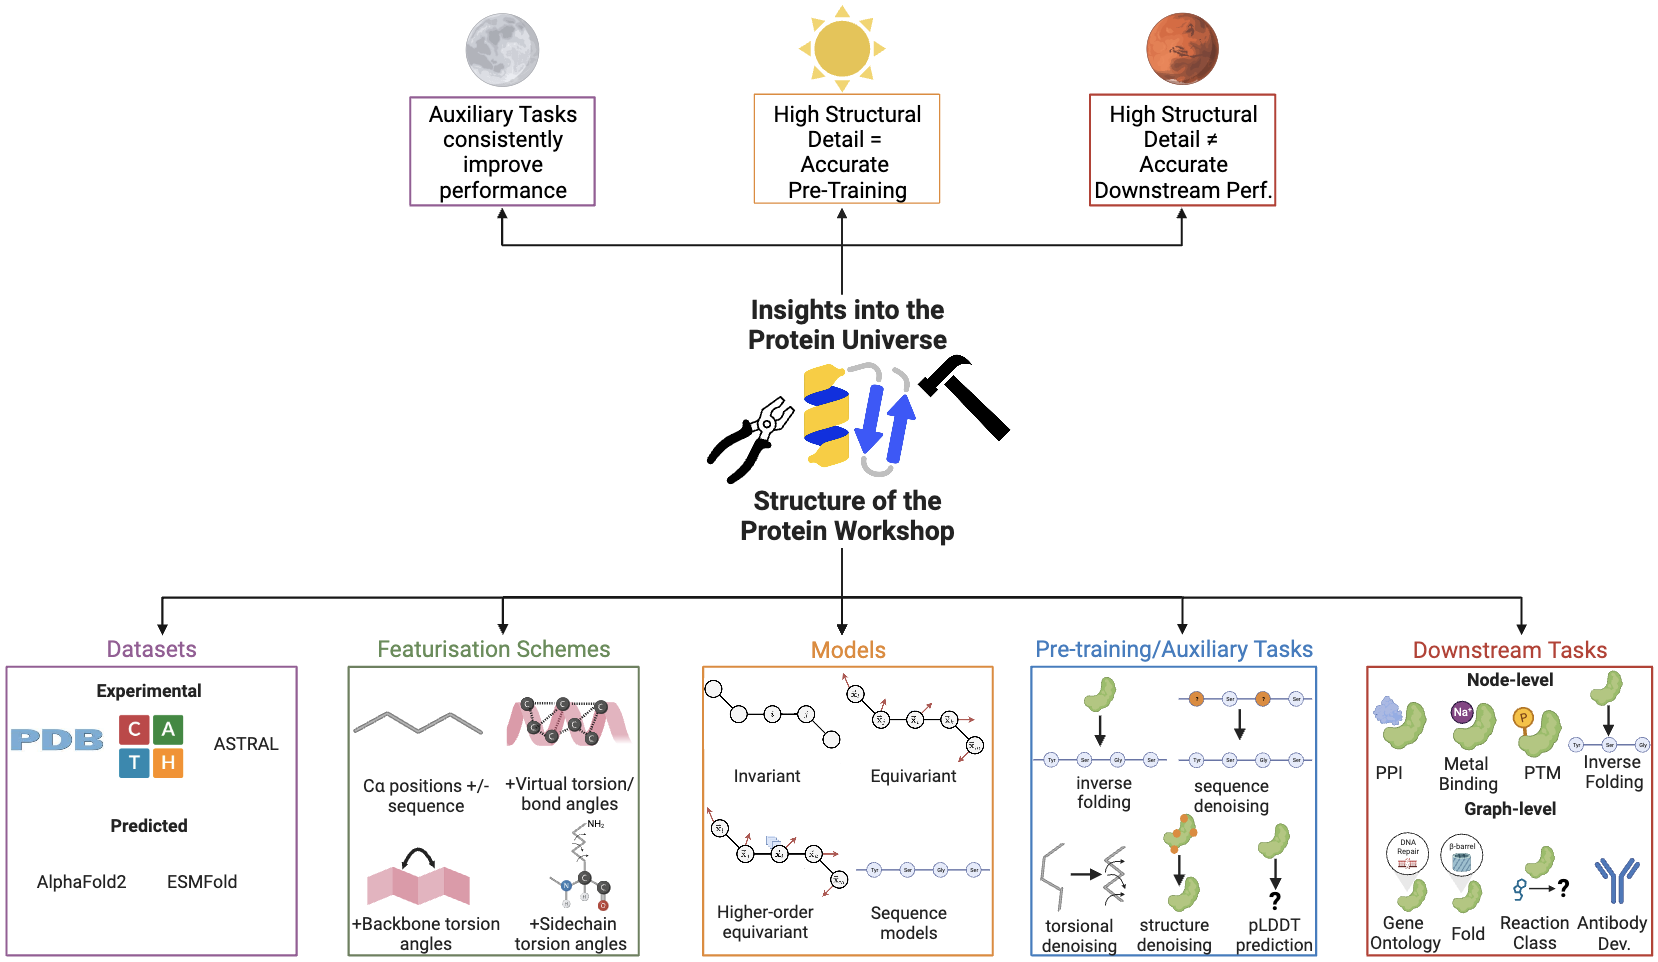
\includegraphics[trim=0 0 0 11.7cm, clip, width=\textwidth]{neurips_data_2023/overview.png}
    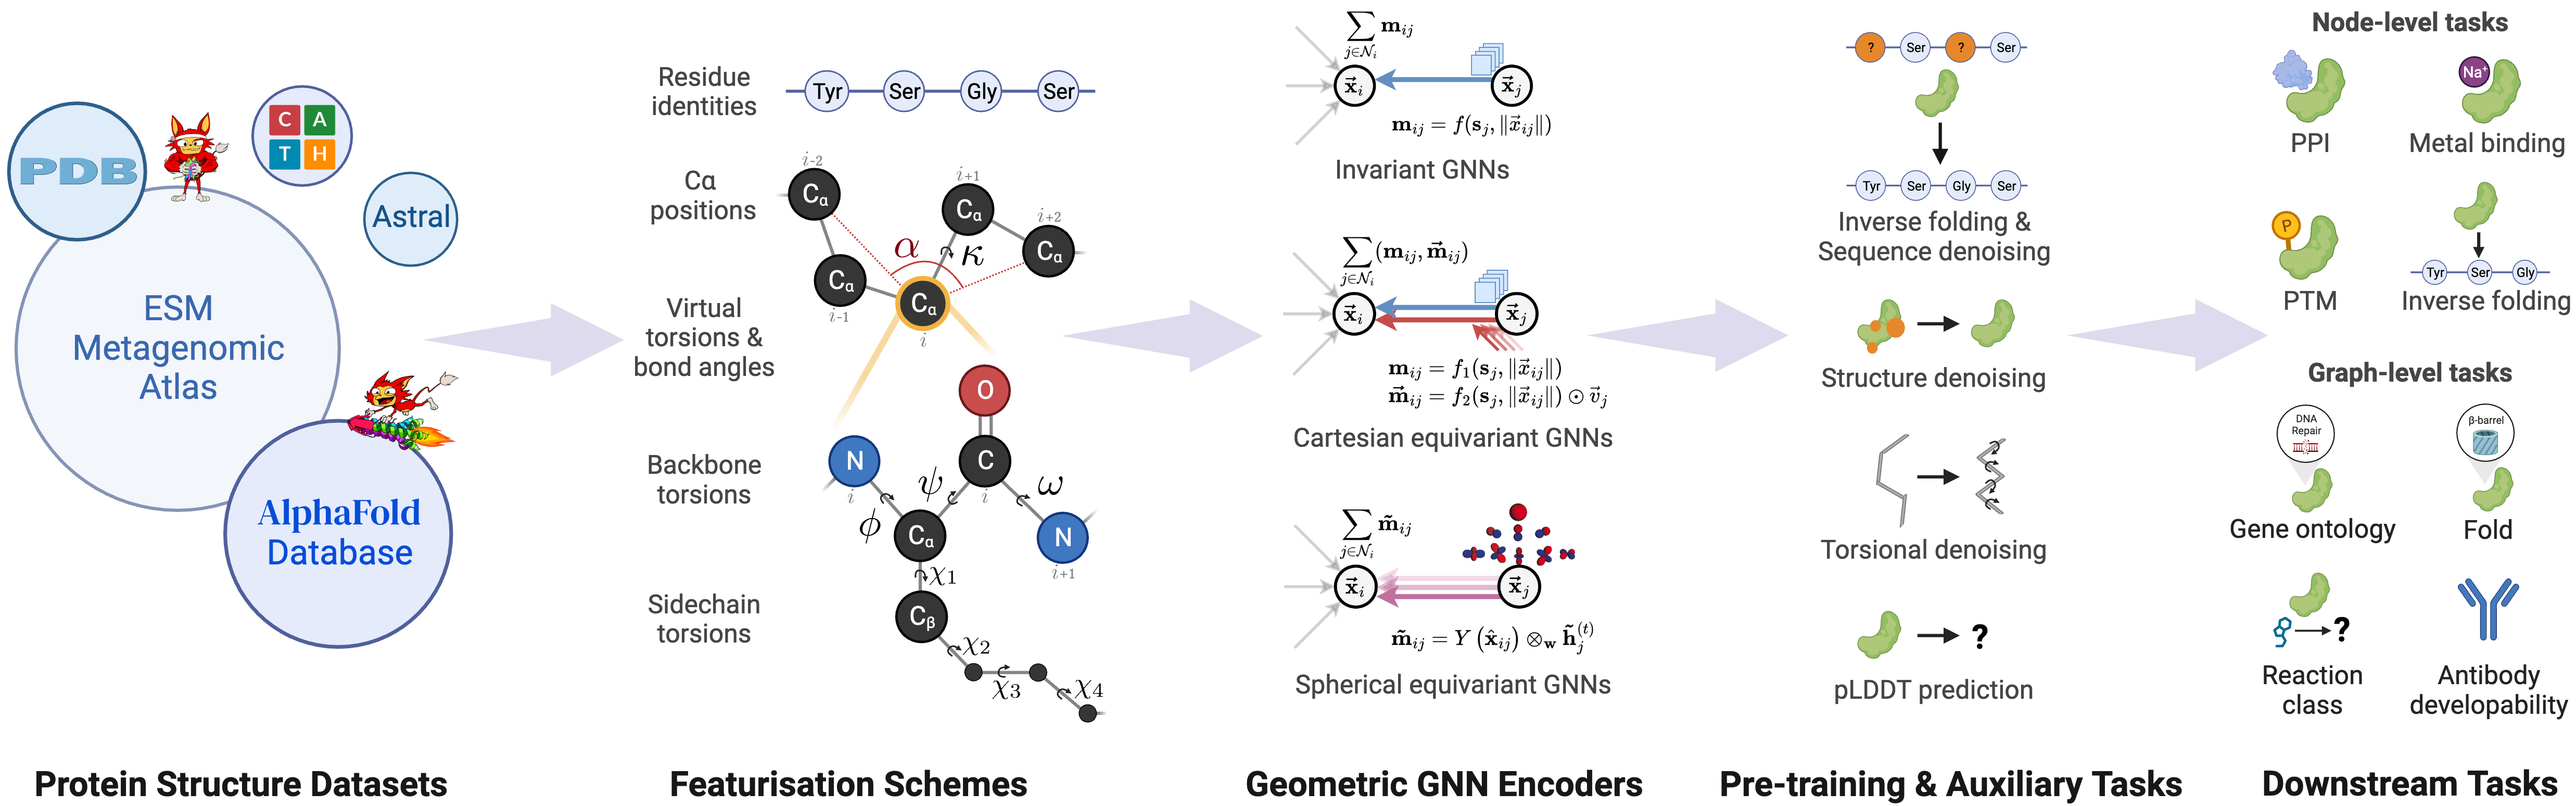
\includegraphics[width=1\textwidth]{iclr_2024/proteinworkshop.jpeg}
    \caption{
    Overview of \emph{ProteinWorkshop}, a comprehensive benchmark suite for evaluating pre-training and representation learning of Geometric GNNs on large-scale protein structure data.
    }
    \label{fig:overview}
\end{figure}

%%%

Our contributions are as follows:\vspace{-5pt}
\begin{itemize}
    \item We curate numerous \emph{structure-based} pretraining and fine-tuning datasets from the literature with a focus on tasks that can enable structural annotation of predicted structures. We compile a highly-modular benchmark, enabling the community to rapidly evaluate protein representation learning methods across tasks, models, and pretraining setups. 
    \item We benchmark Geometric GNNs for representation learning of proteins at different levels of structural granularity (C$\alpha$, backbones, sidechain) and across several classes of models, ranging from general-purpose \citep{schutt2018schnet, satorras2021n} to protein-specific architectures \citep{morehead2024geometry, zhang2023protein}. 
    We are the first to evaluate higher order equivariant GNNs \citep{thomas2018tensor, batatia2022mace} for proteins.
    \item We pretrain and evaluate models on, to our knowledge, the \emph{largest non-redundant} protein structure corpus containing 2.27 million structures from AlphaFoldDB.
    \item Our benchmarks show that sequence denoising-based auxiliary tasks and structure denoising-based pretraining consistently improve Geometric GNNs.
    Moreover, we surprisingly observe that sequence-based pretrained ESM2 \citep{lin2022language} augmented with our structural featurisation matches state-of-the-art GNNs on (super)family fold and gene ontology prediction.
\end{itemize}
% (1) We curate numerous \emph{structure-based} pretraining and fine-tuning datasets from the literature with a focus on tasks that can enable structural annotation of predicted structures. We compile a highly-modular benchmark, enabling the community to rapidly evaluate protein representation learning methods across tasks, models, and pretraining setups. 
% (2) We benchmark protein structure representation learning at different levels of structural granularity (C$\alpha$, backbones, sidechain) and across several families of geometric GNN models, ranging from general-purpose \citep{schutt2018schnet, satorras2021n} to protein-specific architectures \citep{morehead2024geometry, zhang2023protein}. 
% We are the first to evaluate higher order tensor-based equivariant GNNs \citep{thomas2018tensor, batatia2022mace} for protein representation learning.
% (3) We pre-train and evaluate models on, to our knowledge, the \emph{largest non-redundant} protein structure corpus containing 2.27 million structures.
% (4) Our benchmarking study finds that sequence denoising-based auxiliary tasks and structure denoising-based pretraining consistently improve GNN model performance.
% Moreover, we surprisingly observe that sequence-based pretrained ESM2 \citep{lin2022language} augmented with our structural featurisation matches state-of-the-art GNNs on (super)family fold and gene ontology prediction.
% The results of our experiments show, respectively, that sequence denoising-based auxiliary tasks and structure denoising-based pretraining consistently improve the performance of both invariant and equivariant models learning from protein structures. Moreover, we surprisingly observe that sequence-based pretrained models such as ESM2 \citep{lin2022language} provide compelling performance for (super)family fold classification tasks compared to invariant and equivariant GNNs.
